\section{Pipelines}

To convert a dataset depicting a mesh into a visible image on the screen, a series of operations must be carried out. 
This series, akin to the classical pattern designed for leveraging parallel execution of various steps on data, is termed a pipeline.

A pipeline is a framework in which a continuous flow of data undergoes processing through multiple sequential steps. 
As one element progresses to the second step, a new element can begin processing in parallel with the preceding one.
In Vulkan, as well as in computer graphics in general, generating an image on screen from a primitive description involves a series of steps that can be structured into a pipeline.
\begin{figure}[H]
    \centering
    
\includegraphics[width=1\linewidth]{images/pipeline.png}
    \caption{Rendering pipeline}
\end{figure}
The actions performed at each stage of the pipeline can either be predefined by the system or customized by the user.
For historical reasons, algorithms running in the programmable stages of the pipeline are referred to as shaders.

\subsection{Taxonomy}
Various types of pipelines have been defined to handle the generation of 3D images, each serving specific purposes and equipped with distinct sets of fixed functions, input and output descriptions, and programmable stages. Creating a pipeline involves configuring all the parameters required by its fixed functions and connecting it with shaders responsible for the user-defined aspects.
In the latest versions of Vulkan, up to four types of pipelines are supported:
\begin{itemize}
    \item Graphic pipelines.
    \item Ray-tracing pipelines.
    \item Mesh Shading pipelines.
    \item Compute pipelines.
\end{itemize}
The first three are primarily designed for rendering 3D meshes, while the compute pipeline is utilized for general computation purposes, such as general-purpose GPU (GPGPU) tasks. 
Ray tracing and Mesh Shading pipelines may still have limited support as they are relatively recent developments.
Several techniques have been introduced to approximate the rendering equation, including:
\begin{itemize}
    \item Scan-line rendering.
    \item Ray casting.
    \item Ray tracing.
    \item Radiosity.
    \item Monte Carlo techniques.
\end{itemize}
These techniques are closely associated with the types of pipelines that support them.

\paragraph*{Scan-line rendering}

Scan-line rendering is the simplest approximation of the rendering equations.
It treats light sources and objects separately within a scene, where objects reflect light but do not illuminate other objects. 
Consequently, no projected shadows or indirect lighting effects are produced.

In this technique, only the points currently visible to the camera are considered, with lights characterized by having only the emission term in the rendering equation, which can vary in position and direction. 
The vertices of triangles belonging to a mesh are projected onto the screen to determine their corresponding hardware coordinates. 
Subsequently, all pixels belonging to a triangle are enumerated, and for each pixel, the rendering equation is solved.

Inter-reflection between objects is not accounted for, simplifying the integral to a summation over all light sources. 
The geometric term is typically incorporated into the Bidirectional Reflectance Distribution Function (BRDF): 
\[L(x,\omega_r)=L_e(x,\omega_r)+\sum_l L_e(l,\overrightarrow{lx})f_r,(x,\overrightarrow{lx},\omega_r)\]
Visibility in scan-line rendering is determined solely from the perspective of the observer, typically through the z-buffer algorithm. 
Because the visibility term ($V(\cdot)$) of the rendering equation is not considered for lights, scan-line rendering does not generate projected shadows. 
Additionally, it does not account for light emitted by other objects in the scene, nor does it produce effects such as reflection, refraction, or indirect illumination.

However, despite these limitations, scan-line rendering does allow for the incorporation of various types of Bidirectional Reflectance Distribution Function (BRDF) functions.
These BRDF functions can provide detailed descriptions of the materials composing the objects in the scene, enhancing the visual realism despite the simplifications in other aspects of the rendering process.

\section{Vulkan pipeline}
Vulkan facilitates scan-line rendering through a designated pipeline known as the graphics pipeline.
Let's delve into its stages and their respective functions. As outlined in the Vulkan documentation, the graphics pipeline comprises the following structure:
\begin{figure}[H]
    \centering
    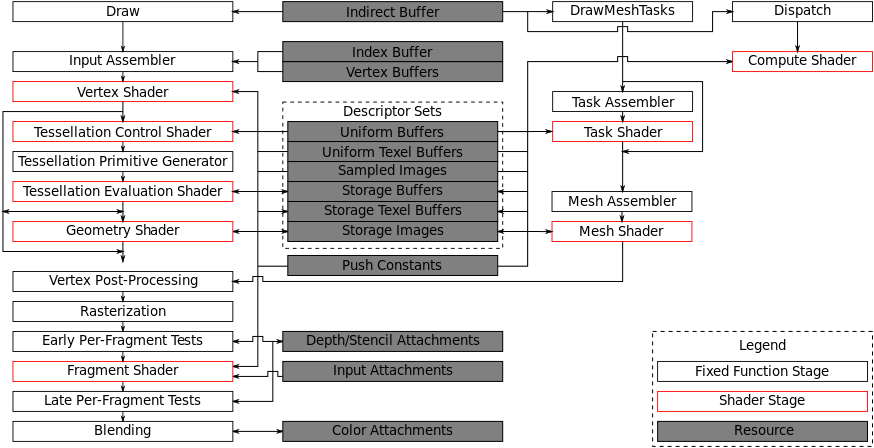
\includegraphics[width=0.75\linewidth]{images/pipelinemesh.png}
    \caption{Vulkan pipeline}
\end{figure}
The graphics pipeline in Vulkan accommodates up to five distinct types of shaders, which define the functionalities of the programmable stages within the pipeline. 
Typically, only the initial and final stages are mandatory. 
In the majority of scenarios, solely the Vertex and fragment shaders are essential to produce an image. 
The tessellation and geometry stages are discretionary; their absence leads the pipeline to disregard these functions and proceed to the subsequent stages.

\paragraph*{Stages}
To draw a triangle using the Vulkan pipeline, you would typically follow these steps:
\begin{enumerate}
    \item \textit{Input assembler}: whenever a draw command is issued, Vulkan creates the vertices by combining all parameters that describe them. 
        If several instances of the same object are used, vertices are replicated as many times as required.
        This stage also decides if we are drawing points, lines, or triangles, using lists or other strip-based approaches.
    \item \textit{Vertex shader}: vertex shaders are executed to perform operations on each vertex. 
        These operations include transforming local coordinates to clipping coordinates by multiplying vertex positions with the corresponding World-View-Projection (WVP) matrix, or computing colors and other values associated with vertices, which will be used in later stages of the process.
    \item \textit{Tessellation}: tessellation is used to increase the resolution of an object. 
    \item \textit{Geometry shader}: geometry shaders can remove or add primitives to the stream, starting from the previously generated elements. 
        In principle, they could perform the same tasks as the tessellation stages. 
        However, due to their generality, implementing these functions in geometry shaders would require more complex code and result in slower performance.
    \item \textit{Rasterization}: rasterization determines the pixels in the frame-buffer occupied by each primitive. 
        These are called fragments, not pixels, since a single pixel on the screen can be computed by merging several fragments to increase the quality of the final image (the so-called anti-aliasing). 
        During these stages, the division by $w$ to transform clipping coordinates into normalized screen coordinates is also performed. 
        
        For example, if the considered basic primitive corresponds to a triangle, the rasterization stage will generate at least a fragment for all the pixels connecting the screen projections of its three vertices. 
        Fragments are usually generated per line, left to right, with respect to the corresponding triangle. 
        This feature is what motivates the scan-line rendering name of this technique.
    \item \textit{Fragment shader}: the final color of each fragment is determined by a user-defined function contained in the fragment shader. 
        This section will use either physically based models or other artistic techniques to produce either realistic or effective images. 
        In other words, it will compute the approximate solution of the rendering equation for the considered pixel.
    \item \textit{Color blending}: finally, the computed colors might either replace the ones already present in the same position, or be combined with them. 
        The latter can be used to implement transparency or other blending effects.
\end{enumerate}

Several important actions occur in the final fixed sections of the pipeline. 
In particular, this is where a few functionalities previously introduced take place: primitives clipping and back-face culling in vertex post-processing. 
Depth testing (z-buffer) and stencil operations in early per-fragment tests.

The pseudocode of a scan-line rendering algorithm is as follows:
\begin{algorithm}[H]
    \caption{Scan-line rendering algorithm}
        \begin{algorithmic}[1]
            \For{each mesh object $A$ in the scene}
                \State{Determine the screen coordinates of each vertex of $t$}
                \For{each visible (passes the back-face culling and clipping) triangle $t$ of $A$}
                    \For{each pixel $x$ of $t$ on screen}
                        \If{pixel $x$ is visible (passes Z-buffer test)}
                            \State{Set the pixel color $C=L_e(x,\omega_r)$}
                            \For{each light $l$ in the scene}
                                \State{Set $C = C + L(l,lx) * fr(x,lx, \omega_r)$}
                            \EndFor{}
                        \EndIf{}
                    \EndFor{}
                \EndFor{}
            \EndFor{}
        \end{algorithmic}
\end{algorithm}

\subsection{Shaders}
In Vulkan, shaders are defined by SPIR-V code blocks. 
SPIR stands for Standard Portable Intermediate Representation, and it is a binary format for specifying instructions that a GPU can run in a device-independent way.
\begin{figure}[H]
    \centering
    
\includegraphics[width=1\linewidth]{images/shaders.png}
    \caption{Shaders}
\end{figure}
Every Vulkan driver converts the SPIR-V code into the binary instructions of their corresponding GPU.\@ 
SPIR-V has been created with the goal of being efficiently converted into instructions for the most popular GPUs, so this process is usually not very expensive from a computational point of view.

Shaders are written in high-level languages, such as:
\begin{itemize}
    \item GLSL\@: OpenGL Shading Language.
    \item HLSL\@: High Level Shading Language (Microsoft DirectX).
\end{itemize}
At development time, the shaders are compiled from their original language to SPIR-V. 
In general, depending on the shader type, the file containing its source code has a different extension. 
Compiled shaders into SPIR-V files have instead the \texttt{spv} extension.

Shaders can be compiled using the glslc tool, which is included in the Vulkan SDK.\@

\section{Ray casting}
Ray casting expands upon scan-line rendering by calculating the visibility function for all point-triangle/light source pairs in the scene. 
It facilitates the inclusion of projected shadows. 
The visibility function is determined by tracing a ray from each considered point to every light source. 
If the ray intersects an object, the light is obstructed, and its contribution to the rendering equation is disregarded. 
Below is the pseudocode for a ray casting rendering algorithm:
\begin{algorithm}[H]
    \caption{Ray casting rendering algorithm}
        \begin{algorithmic}[1]
            \For{each object $A$ in the scene}
                \For{each visible (pass back-face culling and clipping) triangle $t$ of $A$}
                    \For{each pixel $x$ of $t$ on screen}
                        \If{pixel $x$ is visible (pass Z-buffer test)}
                            \State{Set the pixel color $C = 0$}
                            \For{each light $l$ in the scene}
                                \If{light $l$ is not occluded (ray-casting)}
                                    \State{Set $C = C + L(l,lx)\cdot fr(x,l_x, \omega_r)$}
                                \EndIf{}
                            \EndFor{}
                        \EndIf{}
                    \EndFor{}
                \EndFor{}
            \EndFor{}
        \end{algorithmic}
\end{algorithm}
One common real-time technique for ray casting is the utilization of a Shadow Map. 
This map is essentially an image generated from the perspective of the light source, where each pixel's color represents the distance from the point to the light source.
This information is then employed to ascertain whether a pixel is illuminated by the light or obscured.

The shader responsible for rendering computes the distance from the light source to the pixel being rendered and contrasts it with the corresponding distance stored in the shadow map. 
If the computed distance is greater, indicating that the pixel is farther from the light source than the corresponding point in the shadow map, the light contribution is not considered.